\documentclass{article}
\usepackage[parfill]{parskip}
\usepackage{amsmath,amssymb,amsthm}
\usepackage{a4wide}
\usepackage{color}
\usepackage{graphicx}
\graphicspath{{./images/}}
\usepackage[english]{babel}
\usepackage{authblk}

\renewcommand{\epsilon}{\varepsilon}
\newcommand{\bigo}[1]{\mathcal{O}\left(#1\right)}
\newcommand{\note}[1]{\emph{\color{blue}#1}.\\}
\renewcommand{\L}{\mathcal{ L}}
\newcommand{\R}{\mathbb{ R}}
\title{Numerical Homogenization}\author[1]{Ivar Stefansson} 
\author[2]{Omar Richardson} 
\affil[1]{Department of Mathematics and Computer Science, Karlstad University} 
\affil[2]{Department of Mathematics, University of Bergen} 


\begin{document}
\maketitle
\section{Project aim}
\label{sec:project_aim}

We aim to compute effective parameters of a composite material numerically using a finite element simulation implemented in FeNiCS.
Our goal is to explore the relations between the finite element mesh size and the variation in material data.
We consider the Poisson equation with a rapid variation in the diffusion coefficient and explore different solution techniques, focusing in particular on convergence rates and stability.

\section{Model}
\label{sec:model}
We consider a diffusion problem in a composite material. We denote the (periodic) domain with $\Omega \subset \R^d$, for $d\in\{1,2,3\}$. Within this material, we consider unknown quantity $u(x)$, of which the distribution is given by the solution of the Poisson equation:
\begin{equation}
    \begin{split}
        -\nabla \cdot (A_\epsilon(x)\nabla u(x)) &= f(x) \mbox{ for } x \in \Omega,\\
        u(x) &= 0 \mbox{ for } x \in \partial\Omega.
    \end{split}
    \label{eq:model}
\end{equation}

Here, $\epsilon$ is a small positive parameter, denoting the rapid variation of the material.
For diffusivity $A_\epsilon(x)$, we choose a periodic function with a period of order $\epsilon$, like
$$$$
\begin{equation}
   A_\epsilon(x) = \left( 2+\cos\left(\frac{2\pi x}{\epsilon}\right) \right)^{-1}.
   \label{eq:diff_param}
\end{equation}
For $\epsilon \to 0$, it is possible to obtain an homogenized diffusivity, called 'effective diffusion coefficient'.
If time permits, we will extend the model with a diffusion coefficient also varying in the normal length scale, and finally include time dependence in the model as well.

\section{One-dimensional illustration}
\label{sec:onedim}
Let $A_\epsilon$ be defined as in \eqref{eq:diff_param}, let $f(x) = 1$ and let $\Omega = [0,1]$. For this particular choice, we are able to compute the solution to \eqref{eq:model} exactly:
\begin{equation}
    \left( \frac{u'(x)}{2+\cos \left( \frac{2\pi x}{\epsilon} \right)} \right)' = 1
    \label{eq:one_dim}
\end{equation}

Integrating the left hand side of \eqref{eq:one_dim}, dividing by $A_\epsilon$, integrating by parts and substituting the Diriclet boundary condition yields
\begin{equation}
    u(x) = \left( \frac{1}{2} - x \right) \left(2x + \frac{\epsilon}{2\pi}\sin\left(\frac{2\pi x}{\epsilon}\right) \right) + \frac{\epsilon^2}{(2\pi)^2}\left( 1 - \cos \left( \frac{2\pi x}{\epsilon} \right) \right) + x^2
   \label{eq:one_dim_sol}
\end{equation}

\begin{figure}[th]
    \centering
    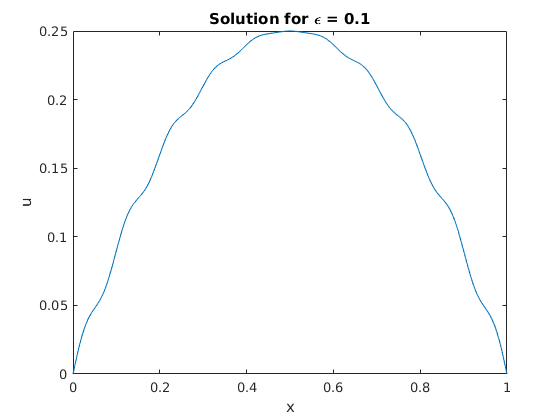
\includegraphics[width=0.5\linewidth]{one_dim_exact.png}
    \caption{Plot of the exact solution to \eqref{eq:one_dim} for $\epsilon=0.1$.}
    \label{fig:one_dim_exact}
\end{figure}

Figure~\ref{fig:one_dim_exact} presents the solution $u$ for $\epsilon = 0.1$. We observe oscillations of size $\bigo{\epsilon}$ and frequency $\bigo{1/\epsilon}$.

From \eqref{eq:one_dim_sol} we can induce that for $\epsilon \to 0$, the frequency of oscillations increases, but their amplitude decreases. This indicates that solving the equation with diffusivity $\lim_{\epsilon\to 0$}A_\epsilon$ results in a smooth solution.

\section{Approximation with FeNiCS}
\label{sec:one_dim_approx}

We implement \eqref{eq:one_dim} in FeNiCS. The weak formulation is straightforward and thus, so is the Python code. An illustration of the numerical approximation is shown in Figure~\ref{fig:one_dim_numerical}. 

\begin{figure}[ht]
    \centering
    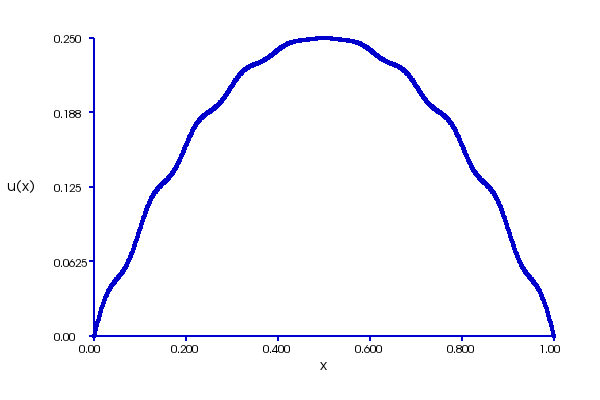
\includegraphics[width=0.5\linewidth]{one_dim_approx.png}
    \caption{Result of FeNiCS simulation of \eqref{eq:one_dim} for $\epsilon=0.1$ and $h = 1/80$}
    \label{fig:one_dim_approx}
\end{figure}

\begin{figure}[ht]
    \centering
    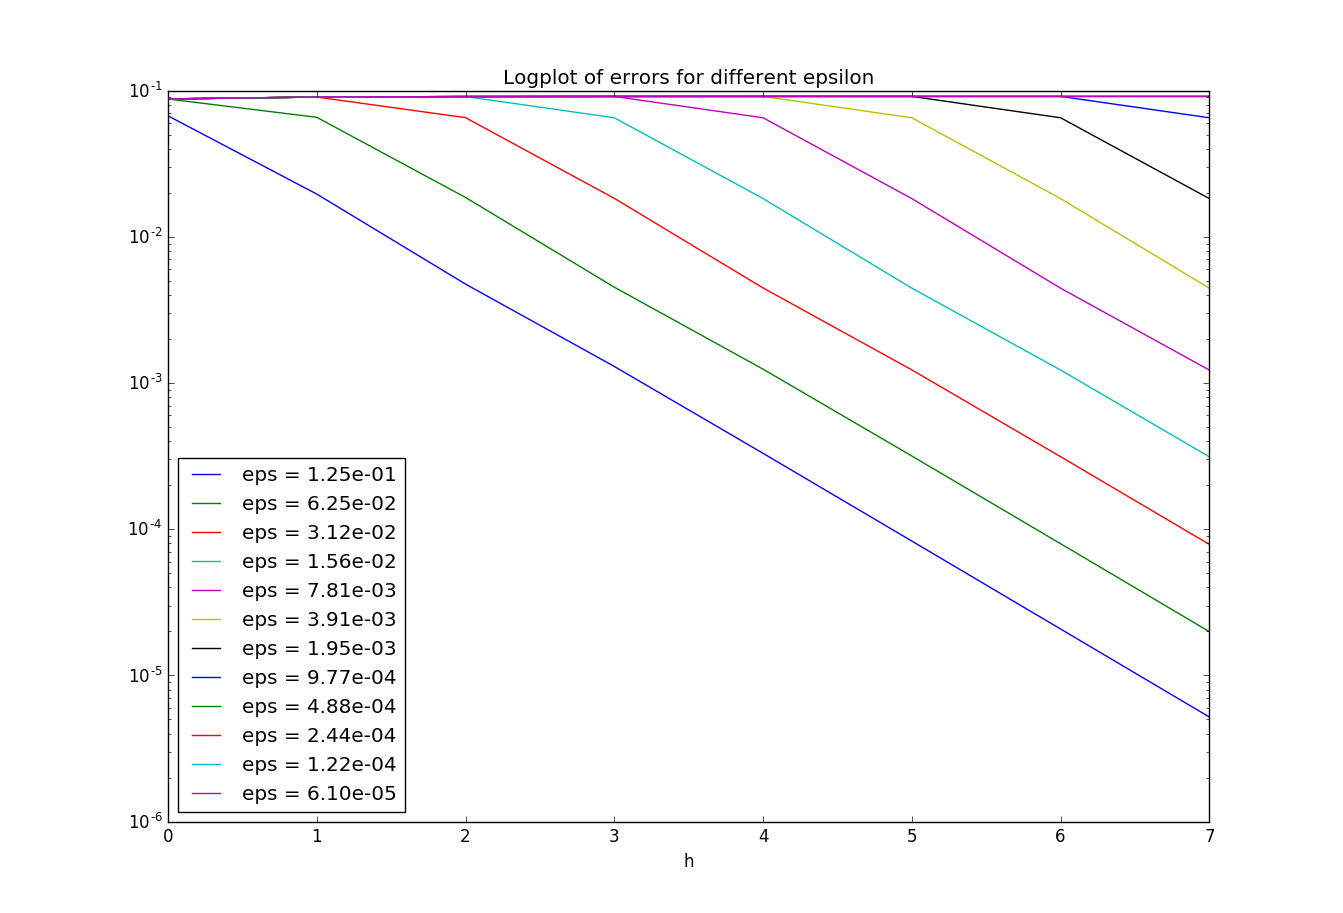
\includegraphics[width=0.5\linewidth]{one_dim_h_eps1.png}
    \caption{Logarithmic plot of error norms for $h\to$, several values of $\epsilon$.}
    \label{fig:one_dim_h_eps1}
\end{figure}

\begin{figure}[ht]
    \centering
    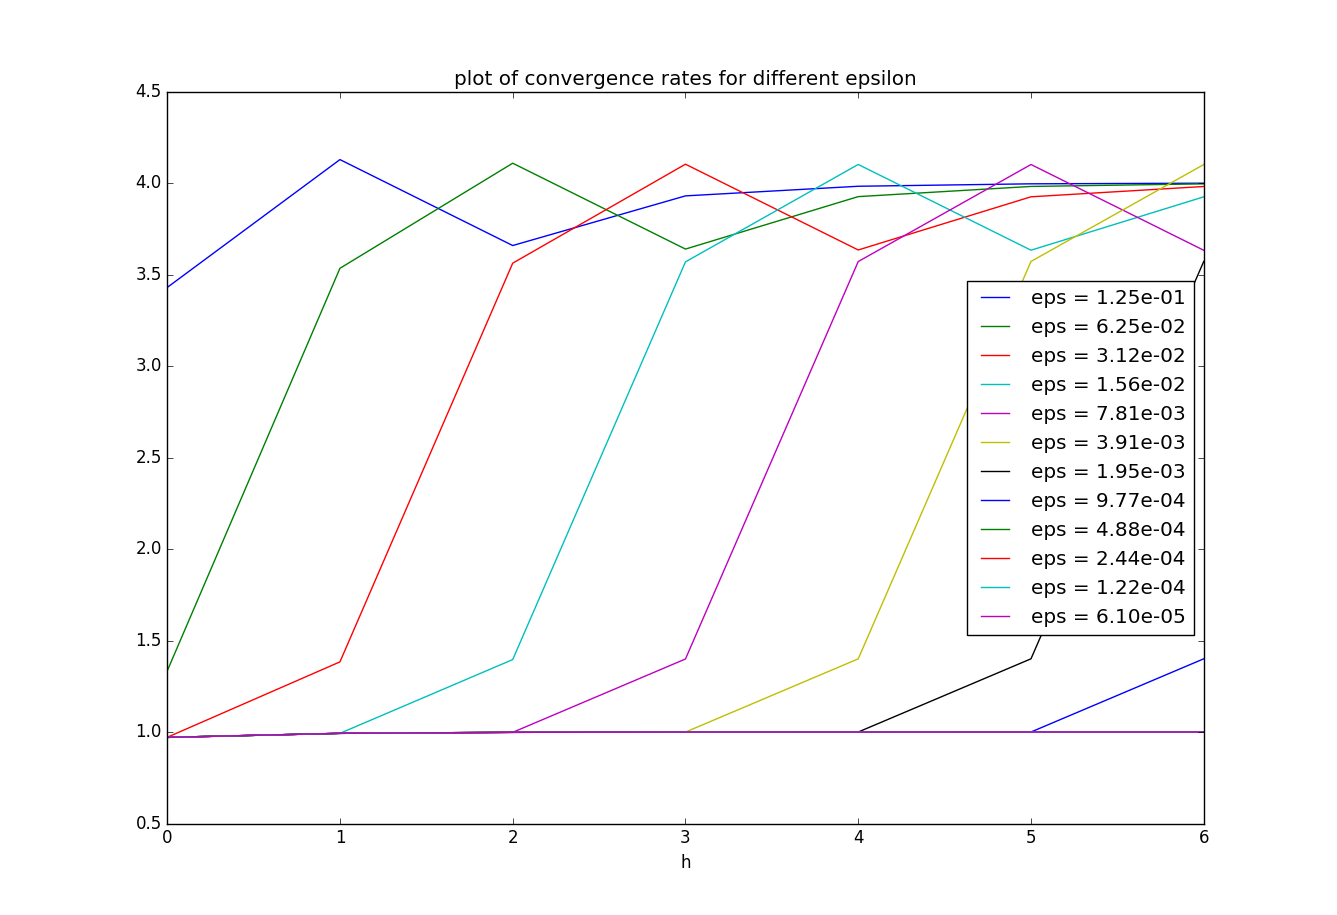
\includegraphics[width=0.5\linewidth]{one_dim_h_eps2.png}
    \caption{Plot of convergence rates, several values of $\epsilon$.}
    \label{fig:one_dim_h_eps2}
\end{figure}

In Figure~\ref{fig:one_dim_h_eps1}, we see that for any $\epsilon$, convergence to the exact solution only occurs for $h \lesssim \epsilon$. Once this grid size restriction is satisfied, we obtain second order convergence as usual. Figure~\ref{fig:one_dim_h_eps2} presents this more clearly.

\section{Effective diffusion coefficients in higher dimensions}
Now, let $\Omega \subset [0,1]^d$ for $d=2,3$. We extend $A_\epsilon$ to multiple dimensions:
\begin{equation}
    A_\epsilon(x) =  \left( 2+\cos\left(\frac{2\pi \sum_{i=1}^dx_i}{\epsilon}\right) \right)^{-1}
\end{equation}
Let $i,j=1,\dots,d$. Let $e_i$ be the $i$th basis vector of $\R^d$. To find the effective diffusion coefficient matrix $(A^*)_{ij}$, we need to solve the corresponding cell problems: find $w_i$ such that
\begin{equation}
    \begin{split}
        -\div_y{A(y)(e_i) + \nabla_2w_i(y)} = 0
    \end{split}
    \label{eq:cell_problem}
\end{equation}
where $w_i$ is periodic in $Y$.

From \eqref{eq:cell_problem}, we obtain the diffusion coefficient by integration:

\begin{equation}
    A^*_{ij} = \int_Y(e_j + \nabla_y w_j)\cdot(e_i + \nabla_y w_i)dy
\end{equation}

\end{document}
